\chapter{Methodology}
This chapter will discuss the methodologies that will be used to address the objectives of the paper. In particular, the chapter is organized as follows: Section \ref{sec:descriptive_stat_method} will discuss the Descriptive Statistics, Section \ref{sec:probability_method} will discuss Probability distributions, Section \ref{sec:stat_graphs_method} will discuss the concept of Histogram, Section \ref{sec:topic_modeling_method} will discuss the concept of Topic Modeling, Section \ref{sec:llm_method} will discuss the concept of Large Language Models, and finally Section \ref{sec:code_setup} will discuss how to implement this in Julia programming language.

Further, the topics discussed here may be self-explanatory for Statisticians, ML researchers or those with Mathematical background. However, for the benefit of readers coming from humanities background, the paper will present the methodology as follows: mathematical formulas are formalized through Definition, Proposition, and Corollary for the sake of brevity, but immediate to these will be an explanation or examples hoping to be simple enough for non-Statistician readers. As a guide, Statisticians or ML researchers can simply read the Definition, Proposition, and Corollary. Whereas for humanities readers, don't stress too much in the said sections, instead use the example or discussions immediate to the said sections to aid with the understanding.
\section{Descriptive Statistics}\label{sec:descriptive_stat_method}
Among the basic statistical methodologies for summarizing information or data is what is known as Descriptive Statistics. From its name, these statistics are meant to convey simple description of the data. For example, \textit{mean}, and \textit{variance} are common statistics used for describing data. The formulas for these statistics are given in the following definitions:
\begin{defnx}[Mean]\label{defn:mean}
Let $x_i, i\in\{1,\cdots,n\}$ where $n\in\mathbb{N}$, then the \textit{mean} of $x_i$s is defined as follows:
\begin{equation}
    \bar{x} = \sum_{i=1}^n x_i, \qquad\text{where}\;x_i \in\mathbb{R}.
\end{equation}
\end{defnx}
\begin{defnx}[Variance]
    Let $x_i, i\in\{1,\cdots,n\}$ where $n\in\mathbb{N}$ and let $\bar{x}$ be the mean defined in Defn. \ref{defn:mean} then the \textit{variance} of $x_i$s is defined as follows:
    \begin{equation}
        \mathbb{V}\text{ar}(x) = \frac{1}{n-1}\sum_{i=1}^n (x_i-\bar{x})^2, \qquad\text{where}\;x_i \in\mathbb{R}.
    \end{equation}    
\end{defnx}
The mean is simply the average of the data points, while the variance is a single number that measures or summarizes the distances of the data points from the mean. The variance therefore gives us an idea of how spread or varied is the data points.
\section{Probability Theory}\label{sec:probability_method}
Another statistical tool to understanding patterns in the data is through the use of Probability distribution. Probability distribution is a model (\textit{see} discussion in Chapter \ref{ch:introduction} for understanding the model). Therefore, Probability distribution is a mathematical formula design to characterize or describe the patterns of a data point--- mathematically represented as a variable (think of this like a placeholder of the data point of the said data). Modeling one variable makes it a univariate model or specifically a univariate probability distribution. Further, modeling more than one variable makes it a multivariate model or a multivariate probability distribution. Formally, the following are necessary definitions to build up on the concept of probability.
\begin{defnx}[Sample Space]
Let $\omega_1,\cdots,\omega_n, \forall n\in\mathbb{N}$ be the list of all possible outcomes of a random event or a phenomena, then the sample space, denoted by $\Omega$, is defined as the collection of all these possible outcomes including the empty set denoted by $\emptyset$.\qed
\end{defnx}
\begin{exmpx}\label{ex:sample_space}
Consider the random phenomenon or event where someone randomly picks a verse from the Qur'\=an, what is the probability that it will be a Meccan \arb{makkiyyaT} or a Medinan \arb{madaniyyaT} verse?

The possible output for such random event is either Meccan or Medinan. Suppose, we let Meccan be denoted by $\omega_1$ and Medinan be $\omega_2$, then the sample space, which is the collection of all possible output is denoted as follows:
\begin{equation}\label{ex_eq:sample_space}
    \Omega:=\{\text{\arb{makkiyyaT}},\text{\arb{madaniyyaT}}\}=\{\text{Meccan}, \text{Medinan},\}=\{\omega_1,\omega_2,\}
\end{equation}
It should be understood that $\emptyset$ is also included in $\Omega$, but is not written for brevity.
\qed
\end{exmpx}
\begin{defnx}[Event]
Let $\Omega=\{\omega_1,\cdots,\omega_n\}, \forall n\in\mathbb{N}$, be the sample space, then an event, denoted here as $\mathscr{A}$, is defined as the subset of the sample space, i.e., $\mathscr{A}\subseteq{\Omega}$.\qed
\end{defnx}
\begin{exmpx}
From Ex. \ref{ex:sample_space}, the event of getting a random verse can be as follows: suppose the first two draws were Meccan and Meccan verses, then mathematically this event can be written as $\mathscr{A}=\{\text{Meccan}\}$. Therefore, $\mathscr{A}$ is a subset of all possible outcomes which is the sample space given in Eq. \ref{ex_eq:sample_space}, and thus $\mathscr{A}\subseteq{\Omega}$. \qed
\end{exmpx}
\begin{defnx}[$\sigma$-algebra]\label{defn:sigma_algebra}
Let $\Omega:=\{\omega_1,\cdots,\omega_n\}, \forall n\in\mathbb{N}$, then the collections of all disjoint partitions, which are the events, are defined as the $\sigma$-algebra or $\sigma$-field, denoted here as $\mathfrak{F}$, and should satisfy the following conditions:
\begin{enumerate}
    \item The empty set $\emptyset\in\mathfrak{F}$
    \item If $\mathscr{A}\in\mathfrak{F}$, then the complement $\Omega\backslash\mathscr{A}$ is also an element of $\mathfrak{F}$
    \item If $\mathscr{A}_1,\mathscr{A}_2,\cdots$ is a countable sequence of sets in \mathscr{A}, then the $\bigcup_{i=1}^{\infty}\mathscr{A}_i$ is also an element of $\mathfrak{F}$
\end{enumerate}\qed
\end{defnx}
\begin{exmpx}
Given the sample space $\Omega:=\{\text{Meccan},\text{Medinan}\}$, the $\sigma$-algebra is $\mathfrak{F}=\{\{\text{Meccan}\},\{\text{Medinan}\},\Omega,\emptyset\}$.\qed
\end{exmpx}
\begin{defnx}[Probability Measure]\label{defn:probability_measure}
Let $\Omega$ be the \textit{sample space}, $\mathfrak{F}$ be the $\sigma$-algebra, $\mathbb{P}$ be the probability measure, then the probability of a set $\mathscr{A}, \mathscr{A}\in\mathfrak{F}$, on the probability space $(\Omega,\mathfrak{F},\mathbb{P})$, denoted by $\mathbb{P}(\mathscr{A})$, satisfies the following properties:
\begin{enumerate}
    \item Non-negativity: For any set $\mathscr{A}, \mathbb{P}(\mathscr{A})\geq 0$
    \item Normalization: $\mathbb{P}(\Omega)=1$
    \item Countable additivity: For any sequence of disjoint sets $\mathscr{A}_1,\mathscr{A}_2,\cdots$ in $\mathfrak{F}$, such that the union $\bigcup_{\forall i \in\mathbb{N}}\mathscr{A}_i$ is also in $\mathfrak{F}$, we have: $\mathbb{P}\left(\displaystyle\bigcup_{\forall i\in\mathbb{N}}\mathscr{A}_i\right)=\displaystyle\sum_{\forall \in\mathbb{N}}\mathbb{P}(\mathscr{A}_i)$
\end{enumerate}
\qed
\end{defnx}

Basically, the idea of Defn. \ref{defn:probability_measure} is to define the concept of "measure" in general sense, although above is a special measure called probability measure. One can think of this probability measure like a tape measure in simple sense. This tape measure has some properties that should be expected for a measurement tool. The first property or condition is that the probability measure has to be positive. Indeed, if we use any tape measure for measuring length, never will someone get a negative measure like -2cm length. It always has to be positive. Further, the second condition to expect is that for this type of tape measure called probability measure, the total measure of all objects available in the given space should be equal to 1. That is, the total is normalized to 1. Think of this like 100\% coverage if we measure all of the objects. Lastly, for any object, this tape measure should be able to measure the object through partitions, such that the measure of the union of these partitions is equal to the sum of the measure of each partition. All of these conditions are logical criteria for a general idea of "measure," although the normalization part above is unique for probability measure. Note that, the concept of proability measure here is should not be confined to measuring length as in the analogy, it should generalize to measuring volume and complex objects in general.
\begin{defnx}[Random Variable]
Let $\Omega$ be the sample space, and $\mathbb{R}$ be the set of all real numbers, then a random variable $X$ is a function defined as $X:\Omega\rightarrow\mathbb{R}$.\qed
\end{defnx}
\begin{exmpx}\label{ex:ayah_prob}
Consider the example of drawing a random verse or \arb[trans]{'ayAt} \arb{'ayAt} again, what is the probability that it will be an \arb[trans]{'ayAt} \arb{'ayAt} from \textit{s\=urah l-baqara}'s \arb[trans]{'ayAt} \arb{A"'yaTu sUraT 'l-baqaraT} or the Chapter of Cow?

The answer to this is 4.59\% probability, this is because there are 286 \arb[trans]{'ayAt} \arb{'ayAt} and there are 6236 verses in the Qur'\=an, so that the probability is $\frac{286}{6236}=0.04586$.
\qed
\end{exmpx}
\begin{exmpx}\label{ex:binom_manual}
To apply the concept so far, consider again Ex. \ref{ex:ayah_prob}, what is the probability of getting 5 \textit{s\=urah l-baqara}'s \arb[trans]{'ayAt} \arb{A"'yaTu sUraT 'l-baqaraT} if we randomly pick 20 \arb[trans]{'ayAt} \arb{'ayAt} in total from the Qur'\=an?\\
\textit{Solution.} The following are given:
\begin{itemize}
    \item $n=20$ independent trials of drawing $x=5$ \arb{'ayAt} from the Qur'\=an
    \item Each trial has two possible outcomes: \arb[trans]{na`am} \arb{na`am} meaning Yes or \arb[trans]{lA} \arb{lA} meaning No. That is, if the \arb[trans]{'ayAt} \arb{'ayAt}  is from the \textit{s\=urah l-baqara} \arb{sUraT 'l-baqaraT} then its \arb{na`am}, otherwise \arb{lA}.
\end{itemize}
Now, the sample space consists of all possible sequences of 20 \arb{na`am} and \arb{lA}. That is,
\begin{align}
    \Omega=\{&
        (\text{\arb{lA}},\text{\arb{na`am}},\text{\arb{lA}},\cdots,\text{\arb{na`am}}),\\
        &(\text{\arb{lA}},\text{\arb{na`am}},\text{\arb{lA}},\cdots,\text{\arb{lA}}),\\
        &\qquad\qquad\vdots\\
        &(\text{\arb{lA}},\text{\arb{lA}},\text{\arb{lA}},\cdots,\text{\arb{lA}})\}.
\end{align}
In total, there are $20^2=400$ possible samples in the sample space $\Omega$. Further, from Ex. \ref{ex:ayah_prob}, the probability of getting a \textit{s\=urah l-baqara}'s \arb[trans]{'ayAt} \arb{A"'yaTu sUraT 'l-baqaraT} is 0.0459 or 4.59\%. Therefore, if we assign \arb{lA}  and \arb{na`am} as either 0 or 1, respectively, then mathematically $\mathbb{P}(X=1)=0.0459$. In addition, the probability of getting an \arb[trans]{'ayAt} \arb{'ayAt} from other \textit{s\=urah} \arb{sUraT} would be $\mathbb{P}(X=0)=1-\mathbb{P}(X=1)=1-0.0459=0.9541$. 

Further, let $Z$ be the random variable for the event of getting $n$ \arb{na`am} from 20 trials, then the problem is equivalent to finding the number of ways to choose 5 positions out of 20 in the collection or set. This can be solved using \textit{combination} formula as shown below:
\begin{align}
    n \choose x &= \frac{n!}{r!(n-r)!}\Rightarrow{20 \choose 5} = \frac{20!}{5!(20-5)!}=15,504. 
\end{align}
That is, there are 15,504 possible cases with 5 positions for \arb{na`am} in a 20 trial. Moreover, in each of these samples 5 has a probability of $\mathbb{P}(X=1)=0.0459$, while the remaining 15 has a probability of $\mathbb{P}(X=0)=0.9541$. So that,
\begin{align}
    \mathbb{P}(Z=5)&=184,756\times\mathbb{P}(X=1)^{5}\times\mathbb{P}(X=1)^{20-5}\nonumber\\
    &=15,504\times0.0459^{5}\times0.9541^{20-5}\nonumber\\
    &=0.0016.
\end{align}
Hence, there is a 0.16\% probability of getting 5 \textit{s\=urah l-baqara}'s \arb[trans]{'ayAt} \arb{A"'yaTu sUraT 'l-baqaraT} when randomly drawing 20 \arb{'ayAt} from the Qur'\=an.
\qed
\end{exmpx}
Note that Ex. \ref{ex:binom_manual} can be solved using a known formula in probability called \textit{Binomial} mass function. The general concept of probability distribution is defined in the following definitions.
\begin{defnx}[Normal Density Function]
Let $Y$ be a random variable and let $\mu\in\mathbb{R}$ and $\sigma\in\mathbb{R}$ be the mean and variance parameters, if $y$ is the random value, then the \textit{Gaussian} or \textit{Normal} density function is given below:
\begin{equation}
    \mathbb{P}(Y=y):=\frac{1}{\sqrt{2\pi\sigma^2}}\exp\left\{-\frac{(y-\mu)^2}{\sigma^2}\right\},\quad\text{where}\;-\infty<y<\infty
\end{equation}
\end{defnx}
\begin{defnx}[Dirichlet Density Function]
Let $\mathbf{Y}$ be a vector random variable with a random value $\mathbf{y}:=[y_1,\cdots,y_k]^{\text{T}}$ and let $\boldsymbol{\alpha}:=[\alpha_1,\cdots,\alpha_k]^{\text{T}}$ be the parameters, then the \textit{Dirichlet} density function is defined as
\begin{equation}
    \mathbb{P}(\mathbf{X}=\mathbf{x};\boldsymbol{\alpha}):=\frac{1}{B(\boldsymbol{\alpha})}\prod_{i=1}^kx_i^{\alpha_i-1},
\end{equation}
where,
\begin{equation}
    B(\boldsymbol{\alpha}):=\frac{\displaystyle\prod_{i=1}^k\Gamma(\alpha_i)}{\Gamma\left(\sum_{i=1}^k\alpha_i\right)}
\end{equation}
\qed
\end{defnx}
\begin{defnx}[Multinomial Mass Function]
Let $\mathbf{X}$ be a vector random variable with a random value $\mathbf{x}:=[x_1,\cdots,x_k]^{\text{T}}$ such that $x_i\geq 0,\forall i \in[1,k]$, let $\boldsymbol{p}:=[p_1,\cdots,p_k]^{\text{T}}$ and $n$ be the parameters, the probability mass function of a Multinomial distribution is 
\begin{align}
    f(x_1,\cdots,x_k;n,p_1,\cdots,p_k):=&\mathbb{P}(X_1=x_1\;\text{and}\;\cdots\;\text{and}\;X_k=x_k)\nonumber\\
    =&\begin{cases}
        \displaystyle\frac{n!}{x_1!\cdots x_k!}p_1^{x_1}\times\cdots\times p_k^{x_k},&\text{when}\;\sum_{i=1}^kx_i=n\\
        0&\text{otherwise},
    \end{cases}
\end{align}
\end{defnx}
\section{Statistical Graphs}\label{sec:stat_graphs_method}
Graphs or plots are data visualization tools that are useful for exploratory data analysis apart from the Descriptive Statistics discussed above. It supplements the Descriptive Statistics findings through shapes visualized in the graphs. Among the popular statistical graphs is the bar graph. An example of this is given in Figure \ref{fig:ayah_word_count}. Other graphs used are the box plots and the density plots which is also in Figure \ref{fig:ayah_word_count}
\subsection{Box, Density, and Histogram Plots}
While most statistical plots are easy to understand like bar graphs and scatter plots, others like Box, Density, and Histogram plots may not be easy to comprehend for someone with no Statistical background. This section will discuss how it is interpreted. Let's use Figure \ref{fig:ayah_word_count}, Figure \ref{fig:ayah_word_count_with_desc} for easy reference in this section.
\begin{figure}[!b]
    \centering
    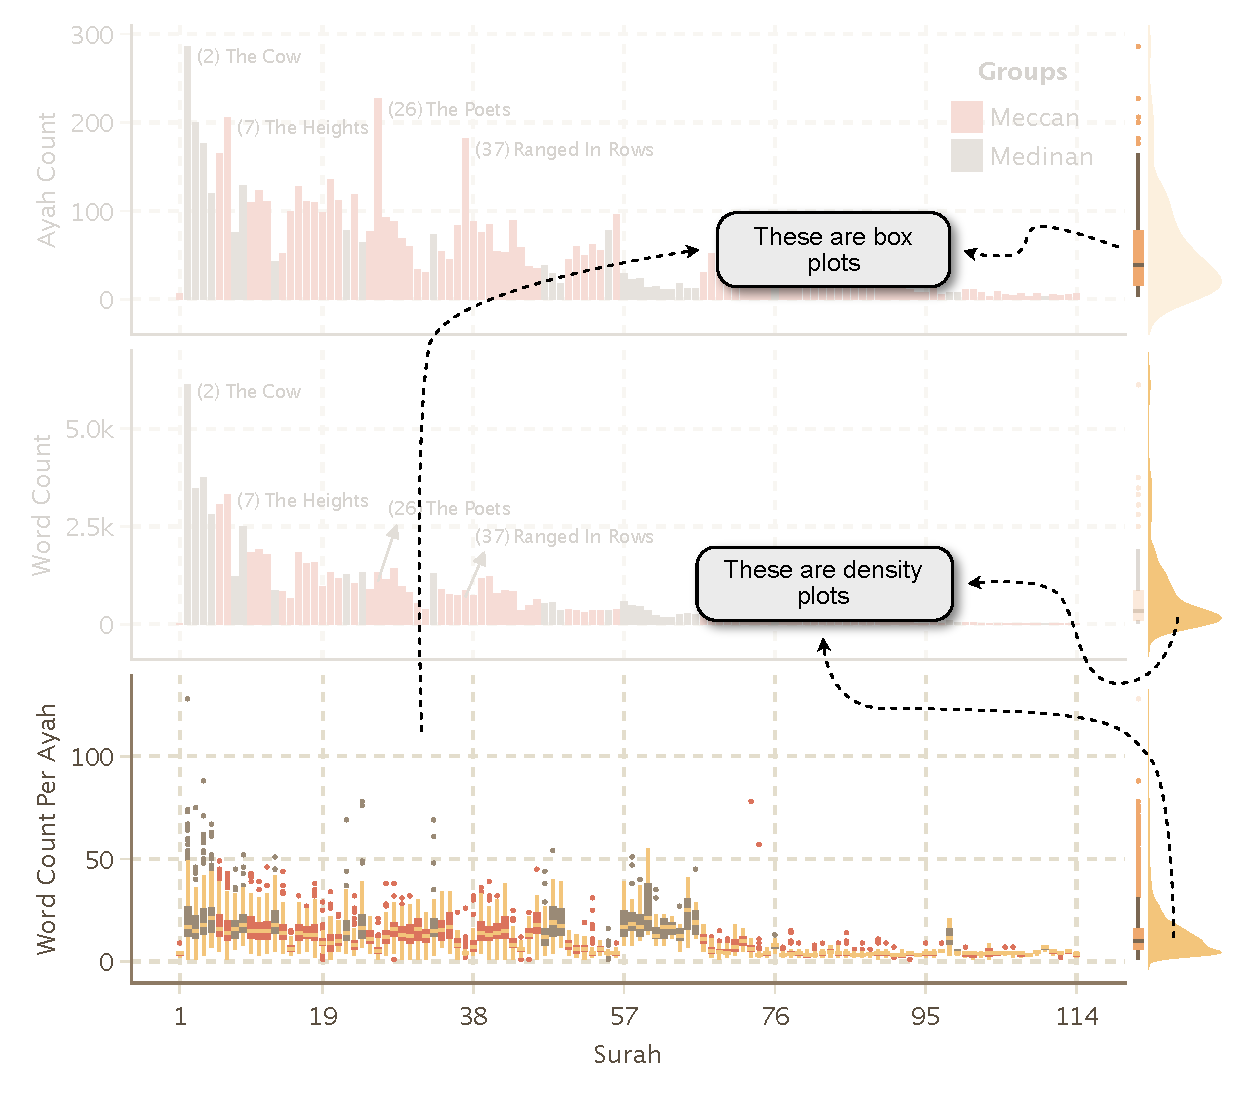
\includegraphics[width=\textwidth]{img/plot1-desc.pdf}
    \caption{Statistics of the words and \arb[trans]{ayAt} \arb{ayAt} (verses) of the Qur'\=an}
    \label{fig:ayah_word_count_with_desc}
\end{figure}

As shown in Figure \ref{fig:ayah_word_count_with_desc}, both the Box and Density plots are tied to each other. This is indeed the case because both are describing the same information but presented in different style of visualization. In fact, Histogram is also used to describe the same information as the Box and Density, and the three are therefore related. So much so, that the three can be put into one graph. As to how to interpret these, readers are referred to for further details \textcolor{red}{[to add reference]}.
\section{Topic Modeling}\label{sec:topic_modeling_method}
As presented in Chapter \ref{ch:introduction}, the first objective is to extract the thematic themes of \textit{s\=urahs} \arb{sUr} with at least 1000 words. In Statistics and Machine Learning, this task is called Topic Modeling. There are several ways to do this, but the popular methodology is to use the Latent Dirichlet Allocation (LDA) discussed in the next section.
\subsection{Latent Dirichlet Allocation}\label{sec:lda}
Latent Dirichlet Allocation (LDA) is a Statistical methodology that is based on Bayesian inference \cite{bayes,laplace1986}. It is a generative probabilisitic model for collection of discrete data such as text corpora \cite{blei2003latent}. The main formula is defined below:
\begin{defnx}[Latent Dirichlet Allocation]
Let $\mathbf{W},\mathbf{Z},\boldsymbol{\theta},\boldsymbol{\varphi}$ be the random variables, and let $\alpha$ and $\beta$ be the hyper-parameters, then the probability of generating a document is
\begin{equation}
    \mathbb{P}(\mathbf{W},\mathbf{Z},\boldsymbol{\theta},\boldsymbol{\varphi})=\prod_{j=1}^m\mathbb{P}(\boldsymbol{\theta}_j;\alpha)\prod_{i=1}^{k}\mathbb{P}(\boldsymbol{\varphi};\beta)\prod_{t=1}^{n}\mathbb{P}(\mathbf{Z}_{j,t}|\boldsymbol{\theta}_j)\mathbb{P}(\mathbf{W}_{j,t}|\boldsymbol{\varphi}_{\mathbf{Z}_{j,t}})
\end{equation}
\end{defnx}
\section{Large Language Models}\label{sec:llm_method}
Generative Artificial Intelligence or GenAI for short has been making waves on its effectiveness to generate texts, images, audio, video, etc. It has elevated humanity to a new level of capability. However, behind this amazing capabilities is that GenAI is by design a mathematical formula that are called \textit{model}. There are several types of \textit{models}, and one of those is the Large Language Model (LLM). The following section will discuss what LLM is and its mathematical formulation.
\subsection{Retrieval-Augmented Generation}
The problem with LLM is that it was only trained on huge but limited data, and is therefore not able to infer what should be the context when asked.
\section{Julia Code Setup}\label{sec:code_setup}
This section will discuss the coding setup. As mentioned in Chapter \ref{ch:introduction}, the main programming language to use is Julia. As such, it is necessary to present where the codes will be stored so that readers are able to reproduce it.

\section{Desktop Application using SvelteKit and Rust}
